% !TEX root = ../thesis.tex
\section{Analýza akustického signálu a jeho parametrizace}
\label{chap:construction:analysis}

Rozpoznávání řeči se věnuje nemalé úsilí již od 50. let 20. století a v~současné době nikoho nepřekvapí téměř bezchybně fungující obecný rozpoznávač souvislé řeči v~mobilních zařízeních.
Pro obecné systémy dokonce existují korpusy s~desítkami, stovkami i více hodinami promluv, které je možné využít při vytváření těchto systémů.
Tyto korpusy ve většině případů obsahují pouze \uv{standardní}\footnote{Slovním spojením \uv{standardní řeč} je myšlena řeč neobsahující výrazné řečové vady, případně jiné formy produkce a často v~nepříliš akusticky náročném prostředí.} řeč.
Pokud se objeví snaha využít systém za specifických podmínek vytvořit nebo ověřit jeho funkčnost (ať už se jedná o rušné prostředí či speciální typy promluv), tak je nezbytné získat potřebná data pořízená za srovnatelných podmínek.

\subsection{Analýza získaných dat}
\label{chap:construction:analysis:data}

Získaný korpus obsahuje přes 10 hodin akustických záznamů promluv a více či méně přesných přepisů\footnote{I přes nemalou snahu a několikastupňovou kontrolu, je téměř jisté, že by nebylo obtížné najít přepis, který obsahuje chybu například ve formě překlepu.}.
V momentě, kdy jsou  k~dispozici data, je možné se zaměřit na specifika EL řeči a případně porovnat se zdravým řečníkem.

Pro potřeby porovnání byl použit začátek promluvy \textit{\uv{Akcie Komerční banky...}}.
Tato promluva je součástí standardní množiny vět používaných při vytváření řečových korpusů na katedře kybernetiky při ZČU.
Tím pádem je  k~dispozici v~relativně velkém množství příkladů pro zdravé řečníky. Tato věta je součástí také korpusu EL řeči.

Na obr. \ref{fig:construction:analysis:comparison} je zobrazen průběh amplitudy a spektrogram vybrané promluvy pro zdravého řečníka (obr. \ref{fig:construction:analysis:comparison:normal}) a EL řečníka (obr. \ref{fig:construction:analysis:comparison:el}).
Už na první pohled je možné zaznamenat určité rozdíly i přesto, že obsah obou promluv je identický.
Prvním rozdílem je délka promluvy.
V~případě zdravého řečníka je v~průměru\footnote{Hodnota odvozena na základě 10 náhodně vybraných promluv ze standardně používaného korpusu na Katedře kybernetiky ZČU.} o celou $1$ vteřinu kratší než v~případě EL řeči.
Tempo řeči je samozřejmě velmi individuální, ale z principu je EL řeč pomalejší.
Navíc z průběhu signálu na obr. \ref{fig:construction:analysis:comparison:el} je patrné, že EL řečník dělá výraznější pauzy mezi jednotlivými slovy promluvy.
To je často způsobené potřebou naplnit jícen vzduchem.
Po TL je dýchání realizováno přes tracheu a pokud nebyl voperován shunt (více v~\ref{chap:cause:treatment:tracheo}), tak je trvale oddělen hrtan a hltan.
I přesto je potřeba, pro produkci některých neznělých fonémů exhalovat vzduch z dutiny ústní.
Zkušený EL řečník to dělá naprosto automaticky, nicméně \uv{polykání} vzduchu zabere nějaký čas.
Nevyhnutelným důsledkem je pak velmi častý výskyt samovolného říhání v~průběhu promluvy\footnote{Fakt, že je říhání jako neřečová událost běžnou součástí téměř každé promluvy, vedl  k~ignorování těchto událostí během anotace.}.

\begin{figure}[htpb]
  \centering
  \begin{subfigure}[b]{0.45\textwidth}
    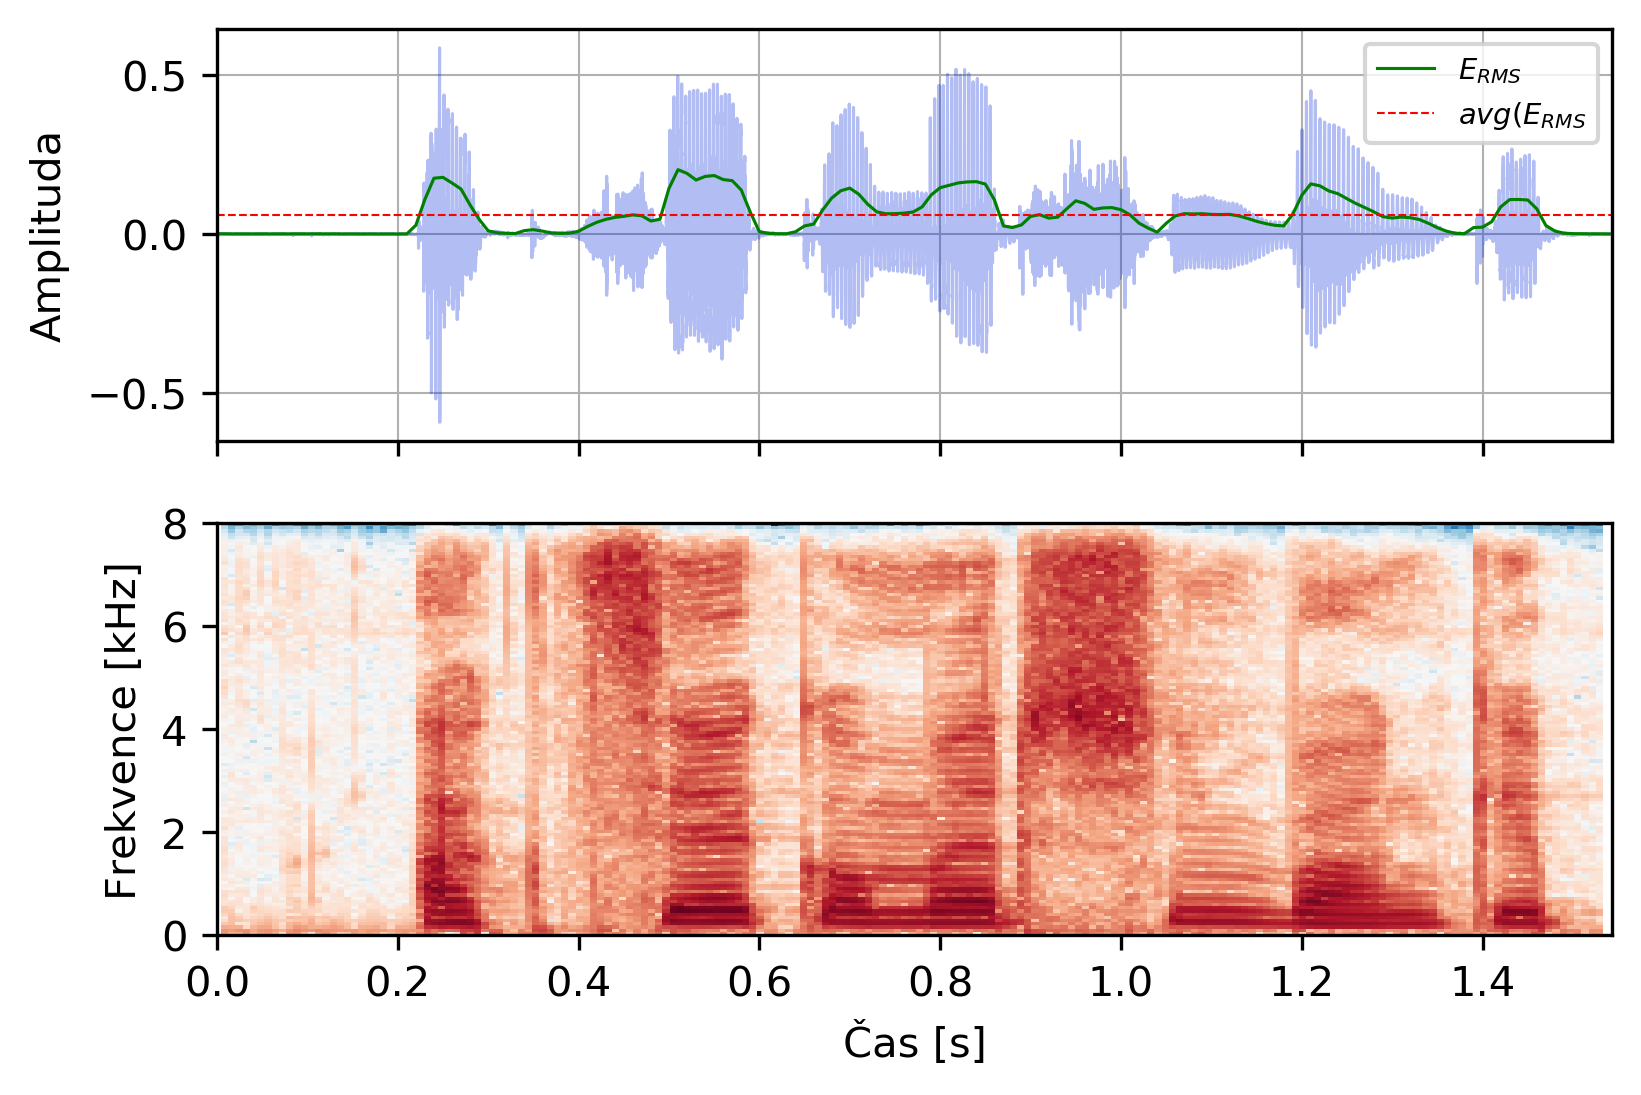
\includegraphics[width=\textwidth]{./ch5-construction/img/energy_spec_normal.png}
    \caption{Zdravý řečník}
    \label{fig:construction:analysis:comparison:normal}
  \end{subfigure}
  %
  \begin{subfigure}[b]{0.45\textwidth}
    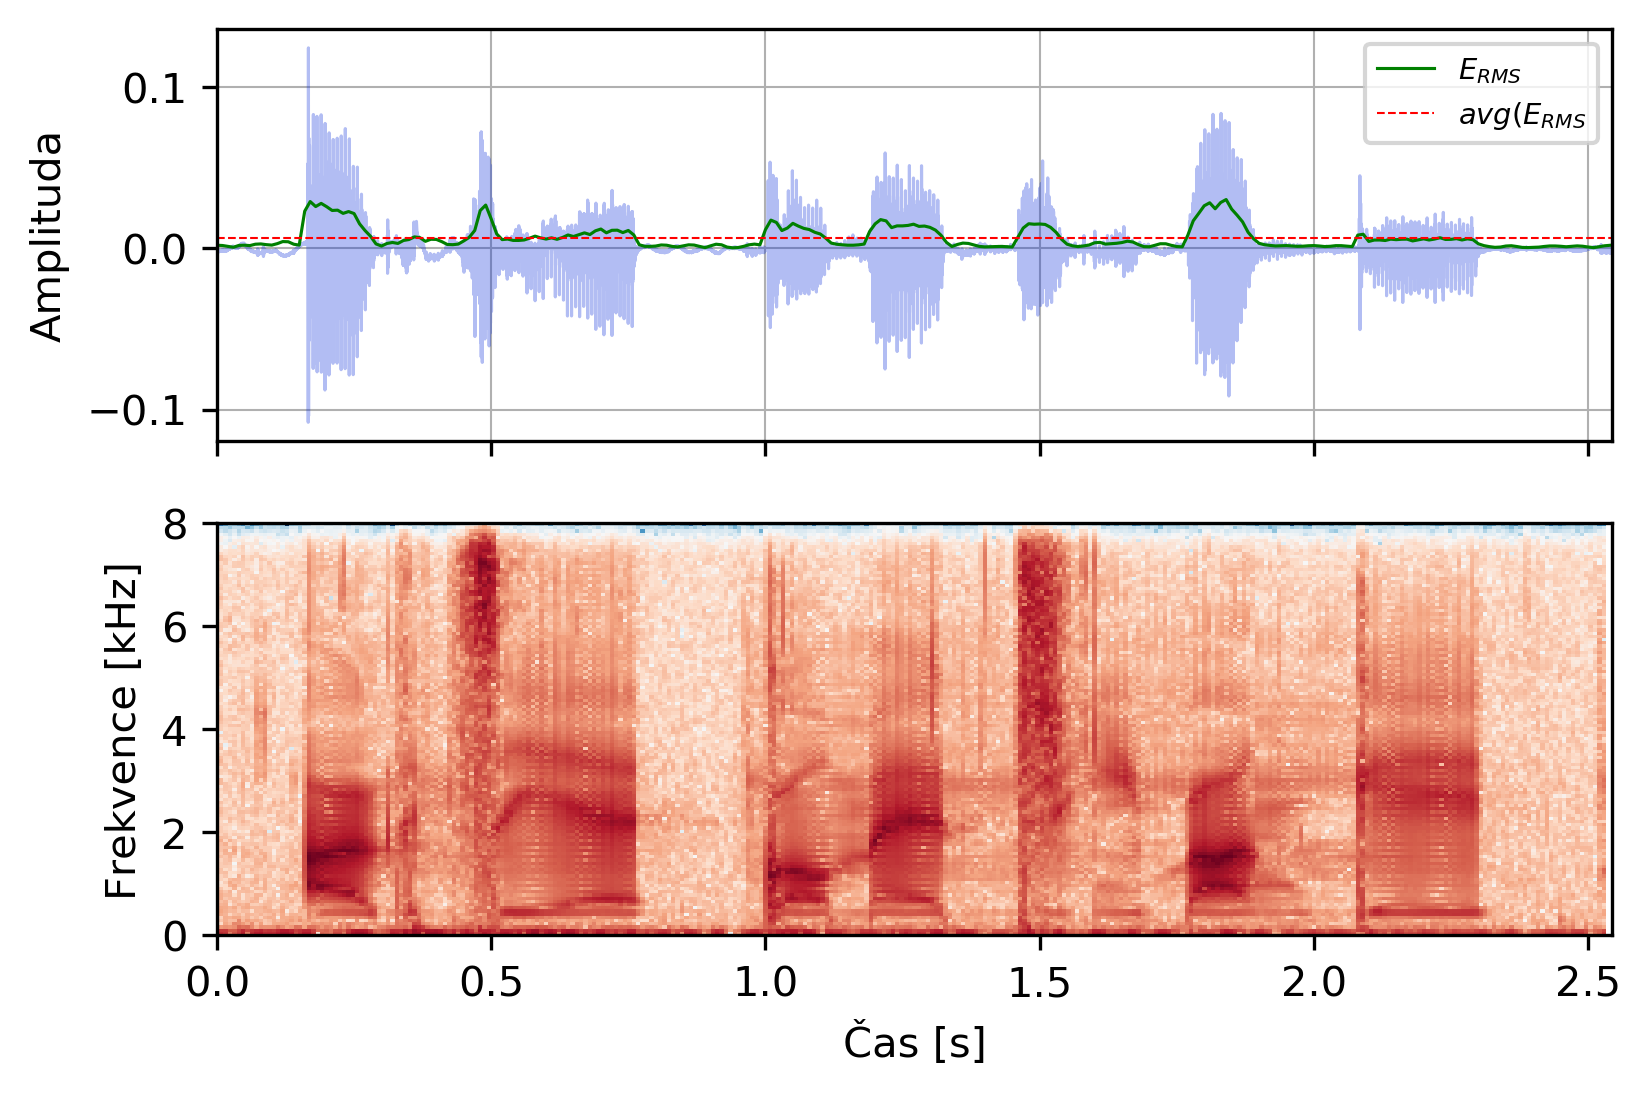
\includegraphics[width=\textwidth]{./ch5-construction/img/energy_spec_el.png}
    \caption{EL řečník}
    \label{fig:construction:analysis:comparison:el}
  \end{subfigure}
  \caption[Průběh a spektrogram promluvy zdravého a EL řečníka.]{Průběh a spektrogram promluvy a vyznačenou energií promluvy zdravého a EL řečníka.}
  \label{fig:construction:analysis:comparison}
\end{figure}

% \begin{figure}[hbpt]
%   \centering
%   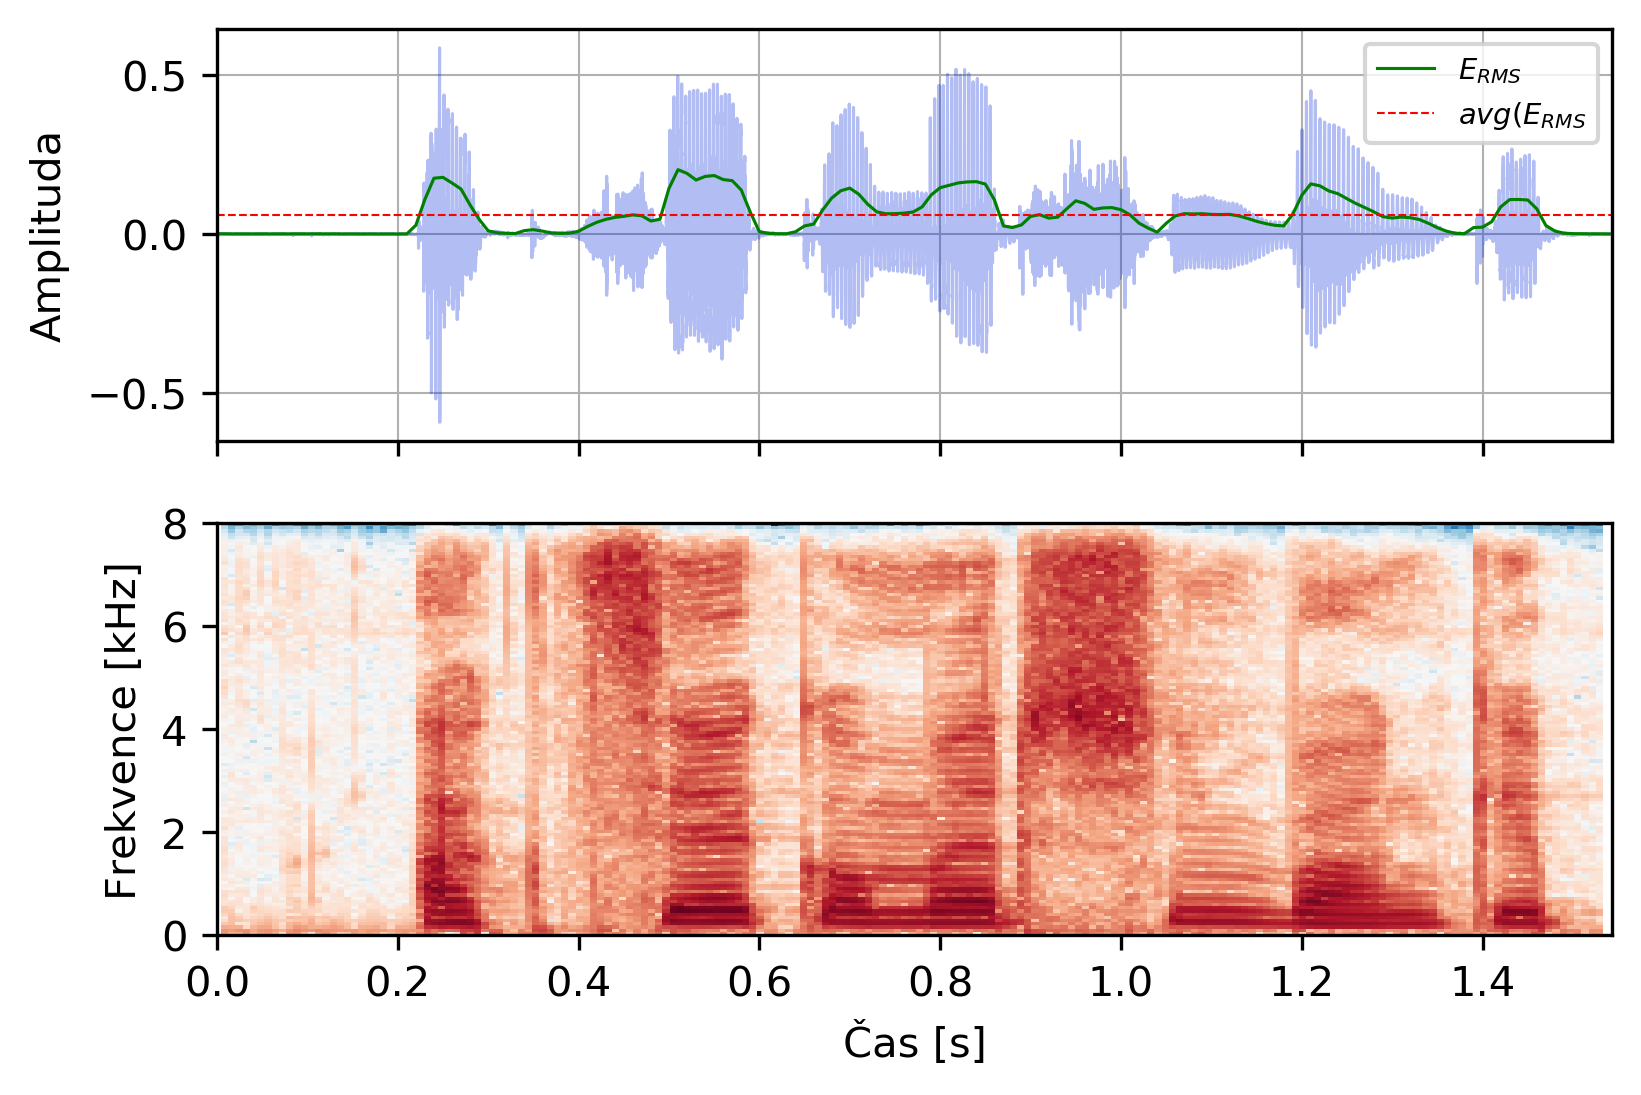
\includegraphics[width=0.9\textwidth]{./ch5-construction/img/energy_spec_normal.png}
%   \caption{Průběh a spektrogram promluvy a vyznačenou energií promluvy.}
%   \label{fig:construction:normal_speech}
% \end{figure}

Svou roli může hrát i snaha správně artikulovat.
Při používání EL je nezbytné, aby bylo produkované řeči alespoň trochu rozumět.
Správná artikulace si žádá svůj čas a není snadné mluvit rychle.
Při nahrávání bylo velmi běžné, že v~průběhu promluvy řečník udělal pauzu, aby mohl lépe umístit EL, protože jeho umístění má velký vliv na kvalitu produkované řeči.
Nicméně je třeba říci, že tempo není pro ASR systémy problém.
%, protože různá délka fonémů je v~relativně snadno modelována, viz část \ref{chap:asr:acoustic}.

Dalším způsobem, jak ukázat rozdíly mezi promluvou zdravého řečníka a řečníka s~EL, je porovnat oba signály ve frekvenční oblasti.
Pro větší názornost jsou na obr.~\ref{fig:construction:spectrogram} zobrazena společně spektra ukázkové promluvy zdravého řečníka (\ref{fig:construction:spectrogram:normal}) a toho s~EL (\ref{fig:construction:spectrogram:el}), přičemž obsah obou promluv je identický.
Prvním markantním rozdílem je mnohem významnější zastoupení šumu v~promluvě řečníka s~EL v~úsecích \uv{ticha}, viz obr. \ref{fig:construction:spectrogram:el}.
To je nepochybně způsobeno samotným EL, který řečník mezi jednotlivými slovy nevypíná.
Přítomnost šumu se projeví zejména na průběhu energie (viz obr. obr. \ref{fig:construction:el_speech}), zejména před prvním a druhým slovem promluvy.
%Na obr. \ref{fig:construction:el_speech} je zřetelně patrný, zejména na průběhu energie, šum před prvním a druhým slovem promluvy.
Zajímavá je přítomnost šumu v~celém frekvenčním spektru, přestože EL produkuje konstantní buzení, které je ve spektru (obr. \ref{fig:construction:spectrogram:el}) reprezentováno výraznou souvislou linií na nízkých frekvencích.
Přítomnost šumu na vyšších frekvencích je způsobena umístěním mikrofonu, který je nalepen přímo na pokožku, a tím pádem snímá namodulované vibrace přenášené měkkou tkání.
Tato hypotéza byla potvrzena v~dalších etapách nahrávání, kde byl použit studiový mikrofon vzdálený od úst minimálně 15 cm, toto bude podrobněji bude popsáno v~části \ref{chap:realisation:corpus}.
Nicméně z pohledu použitelnosti nějakého budoucího systému je nezbytné počítat i se situací, kdy mikrofon zaznamenává i vibrace přenášené tkání.

Dalším významným rozdílem v~promluvě EL řečníka je absence vyšších frekvencí u většiny produkovaných fonémů.
Absence vyšších frekvencí se dá vysvětlit nejen použitím EL, kde samotný EL má vždy konstantní frekvenci buzení, ale i tím, že nedochází  k~modulaci ve všech dutinách vokálního traktu.
Výjimku tvoří afrikáty $/c/$ a $/\check{c}/$, u kterých jsou hlasivky (u zdravého jedince) v~klidu, a vznikají uvolněním nahromaděného vzduchu v~dutině ústní\footnote{Nahromadění vzduchu je realizováno přitisknutím jazyka  k~přední/zadní části horního patra.} \cite{Psutka2006}.
U řečníka po TL není mechanismus produkce těchto fonémů žádným způsobem ovlivněn.
%U těchto fonémů není, u  řečníka po TL, mechanizmus produkce těchto fonémů ovlivněn.
Problémem teoreticky může být zdroj vzduchu, jelikož jej z plic není možné dostat do dutiny ústní, ale jak už bylo zmíněno (a spektrogram to potvrzuje), zkušený uživatel EL se dokáže adaptovat.

 Nicméně nejdůležitější frekvenční složky, zajišťující srozumitelnost promluvy, se vyskytují ve frekvenčním pásmu od $1\ kHz$ do $3\ kHz$.
 Vyšší frekvence se podílejí a priori na zabarvení hlasu.

\begin{figure}[htpb]
  \centering
  \begin{subfigure}[b]{0.4\textwidth}
    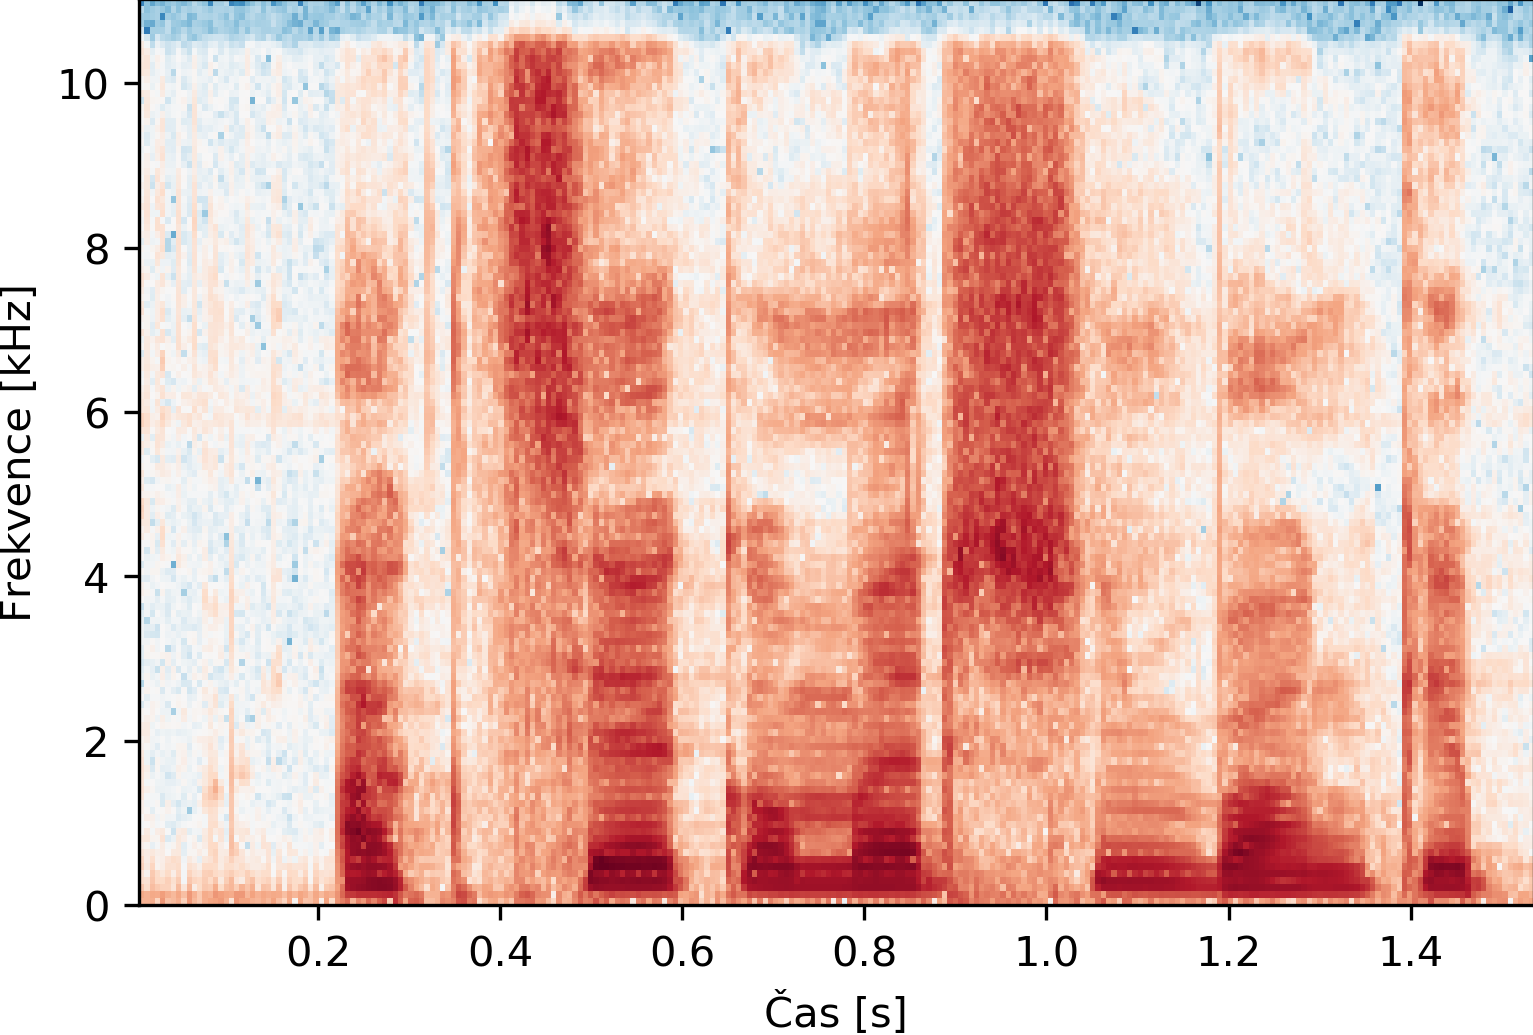
\includegraphics[width=\textwidth]{./ch5-construction/img/spectrogram_normal.png}
    \caption{Zdravý řečník}
    \label{fig:construction:spectrogram:normal}
  \end{subfigure}
  %
  \begin{subfigure}[b]{0.4\textwidth}
    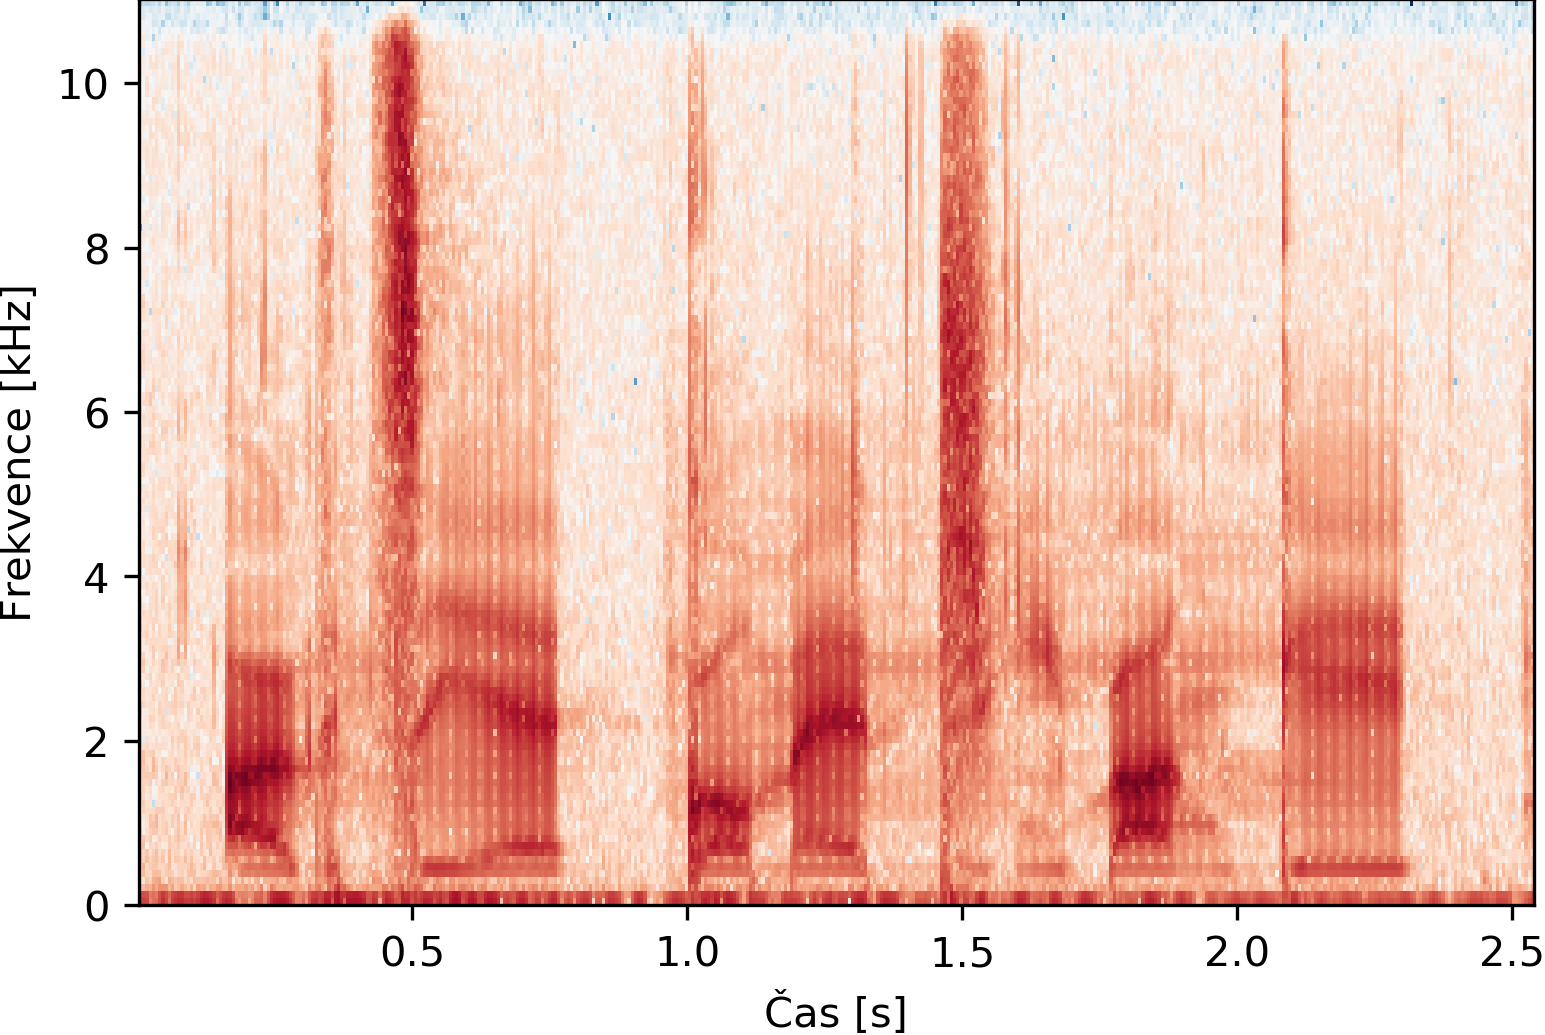
\includegraphics[width=\textwidth]{./ch5-construction/img/spectrogram_el.png}
    \caption{EL řečník}
    \label{fig:construction:spectrogram:el}
  \end{subfigure}
  \caption{Spektrogram promluvy \uv{Akcie Komerční banky} dvou řečníků.}
  \label{fig:construction:spectrogram}
\end{figure}

Dalším způsobem, jak porovnat promluvy zdravého řečníka  a EL řečníka, je na úrovni analýzy jednotlivých fonémů.
Na obr. \ref{fig:construction:phonemes:k} - \ref{fig:construction:phonemes:c} jsou zobrazeny průběhy amplitud jednotlivých fonémů v~čase\footnote{Hodnoty času odpovídají časům výskytu v~původní promluvě.} pro fonémy $/k/$, $/g/$ a $/\check{c}/$.
V případě $/k/$ a $/g/$ (obr. \ref{fig:construction:phonemes:k} a \ref{fig:construction:phonemes:g}) se jedná o okluzivy, konkrétně $/k/$ je kategorizováno jako neznělá ploziva a $/g/$ jako znělá ploziva.
Tyto fonémy obecně vznikají v~důsledku uzavření vydechovaného proudu vzduchu pomocí artikulačních orgánů, což se projeví jako krátká pauza (tzv. okluze).
Po té následuje náhlé jednorázové uvolnění překážky a únik nahromaděného vzduchu, tzv. exploze \cite{Psutka2006}.
Takto popsáno to samozřejmě funguje u zdravého jedince.
V případě EL řečníka je pro jejich produkci využíván stejný mechanizmus, ale vydechovaný vzduch pochází z hltanu.
Dalším rozdílem je samozřejmě absence hlasivek.

Foném $/k/$ je tedy zástupcem skupiny neznělých fonémů.
Ty se vyznačují tím, že do jejich produkce nevstupují hlasivky, jsou v~klidu.
Zdrojem buzení je tedy šum, viz část \ref{chap:asr}.
Pokud se podíváme na průběh amplitudy v~čase u zdravého řečníka (obr. \ref{fig:construction:phonemes:k:normal}), není zde vidět žádný periodický signál.
Hlasivky jsou tedy opravdu v~klidu.
Oproti tomu u EL řečníka (obr. \ref{fig:construction:phonemes:k:el}) je jasně patrné, že je zde přítomno aktivní buzení vytvořené EL.
Ve frekvenční oblasti je zobrazeno tzv. amplitudové spektrum, které znázorňuje závislost amplitudy signálu na frekvenci.
V případě zdravého řečníka odpovídá vývoj předpokladům.
Není zde žádná výrazná frekvence a také nedochází k~výraznému útlumu.
Přestože se v~obou případech jedná o stejný foném, je z časového i frekvenčního průběhu amplitudy zřejmé, že parametry signálu se u obou řečníků diametrálně liší.

\begin{figure}[htpb]
  \centering
  \begin{subfigure}[b]{0.45\textwidth}
    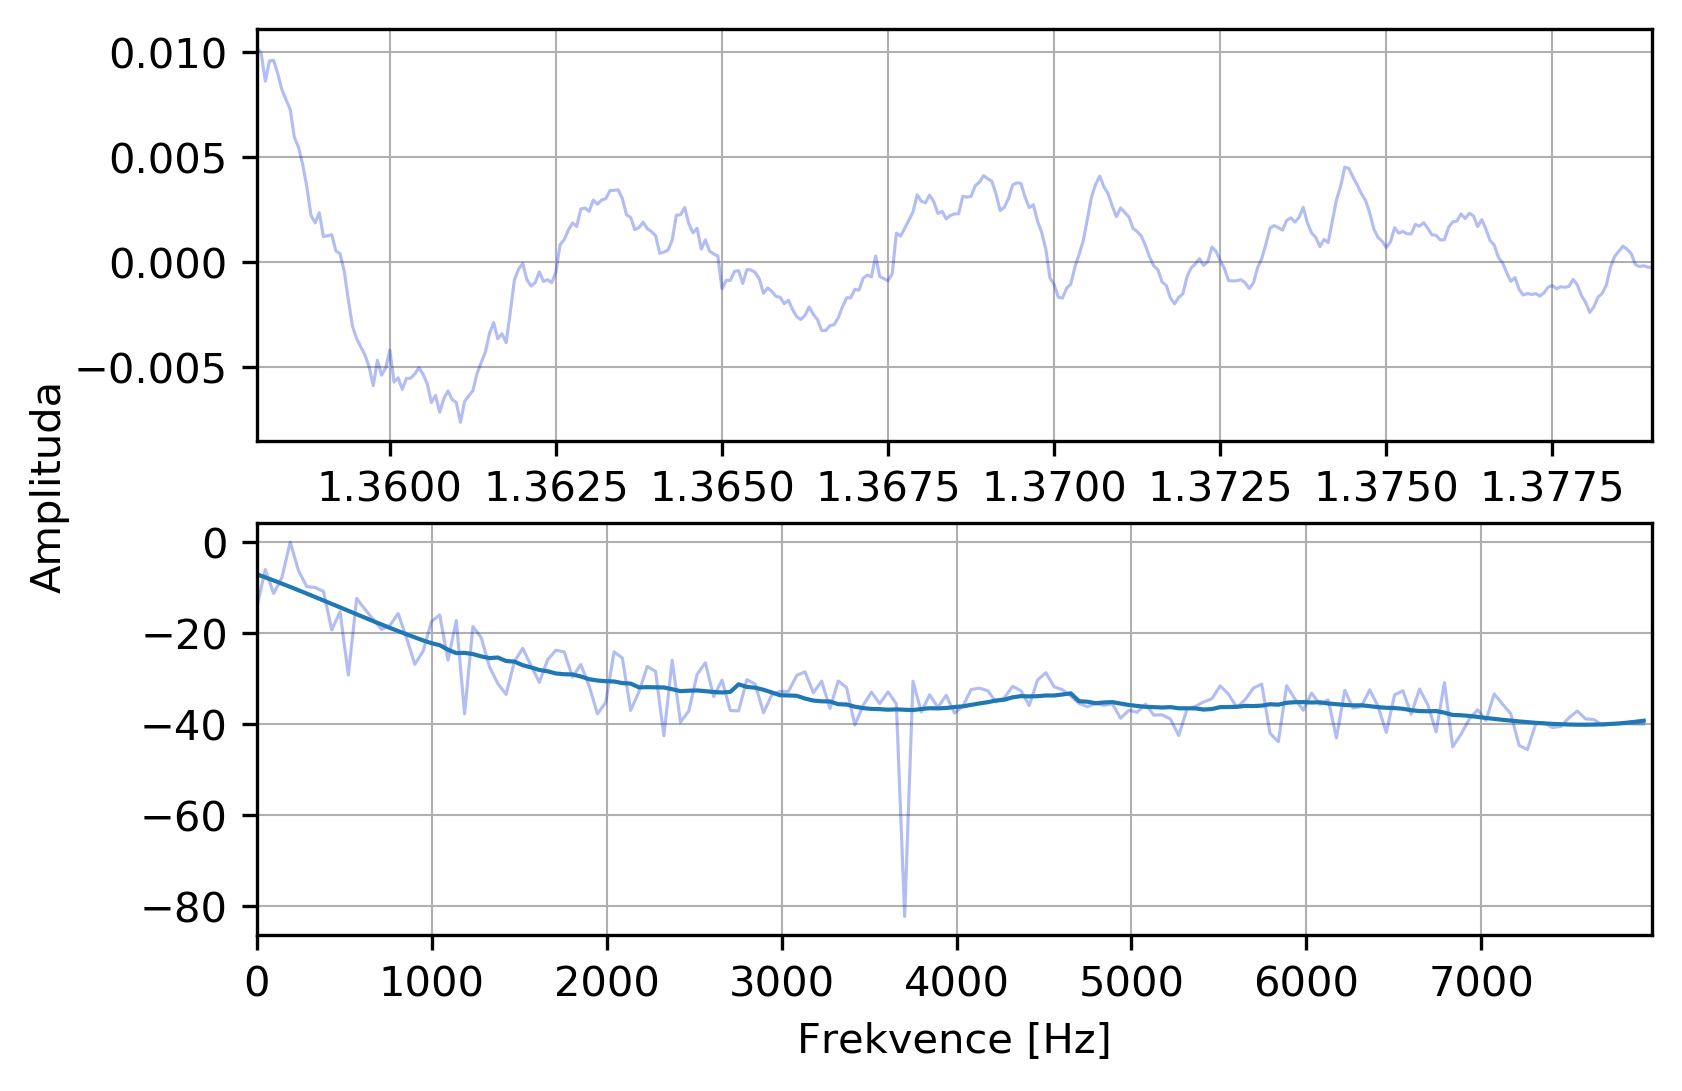
\includegraphics[width=\textwidth]{./ch5-construction/img/signal-normal_k.png}
    \caption{Zdravý řečník}
    \label{fig:construction:phonemes:k:normal}
  \end{subfigure}
  %
  \begin{subfigure}[b]{0.45\textwidth}
    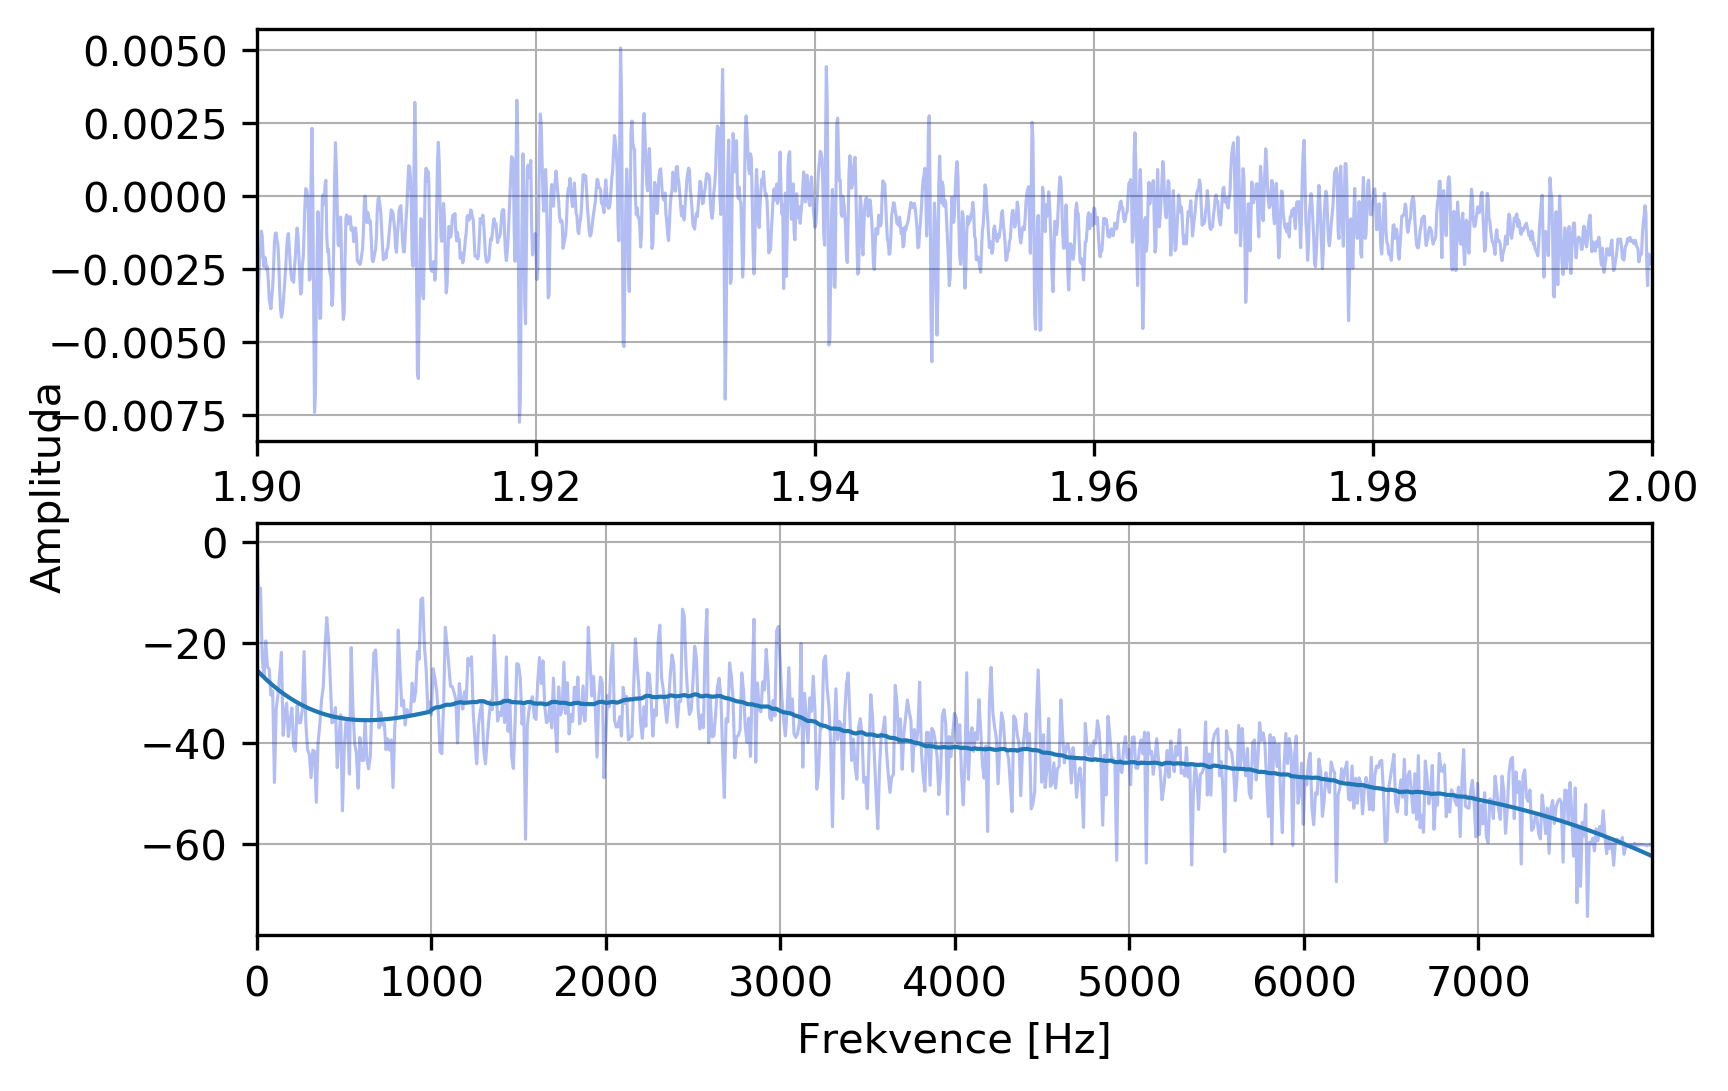
\includegraphics[width=\textwidth]{./ch5-construction/img/signal-el_k.png}
    \caption{EL řečník}
    \label{fig:construction:phonemes:k:el}
  \end{subfigure}
  \caption[Průběh amplitudy fonému $/k/$ zdravého a EL řečníka.]{Průběh amplitudy $/k/$ v~časové a frekvenční oblasti fonému u~zdravého a EL řečníka.}
  \label{fig:construction:phonemes:k}
\end{figure}

Jako druhý ukázkový foném byl vybrán $/g/$.
Jedná se o znělou plozivu.
Při produkci znělých fonémů hrají velký vliv hlasivky, protože jsou zdrojem buzení.
Z~obr. \ref{fig:construction:phonemes:g:normal} je toto buzení zřetelné ve formě periodického průběhu amplitudy.
U EL řečníka (obr. \ref{fig:construction:phonemes:g:el}) je také vidět periodický signál, ale úplně jiného charakteru.
Svým způsobem dost podobný tomu, který je zřetelný u fonému $/k/$.
Rozdíl je zřetelný i ve frekvenční oblasti, kdy u EL řečníka nedochází  k~útlumu ve střední oblasti frekvenčního spektra.

\begin{figure}[htpb]
  \centering
  \begin{subfigure}[b]{0.45\textwidth}
    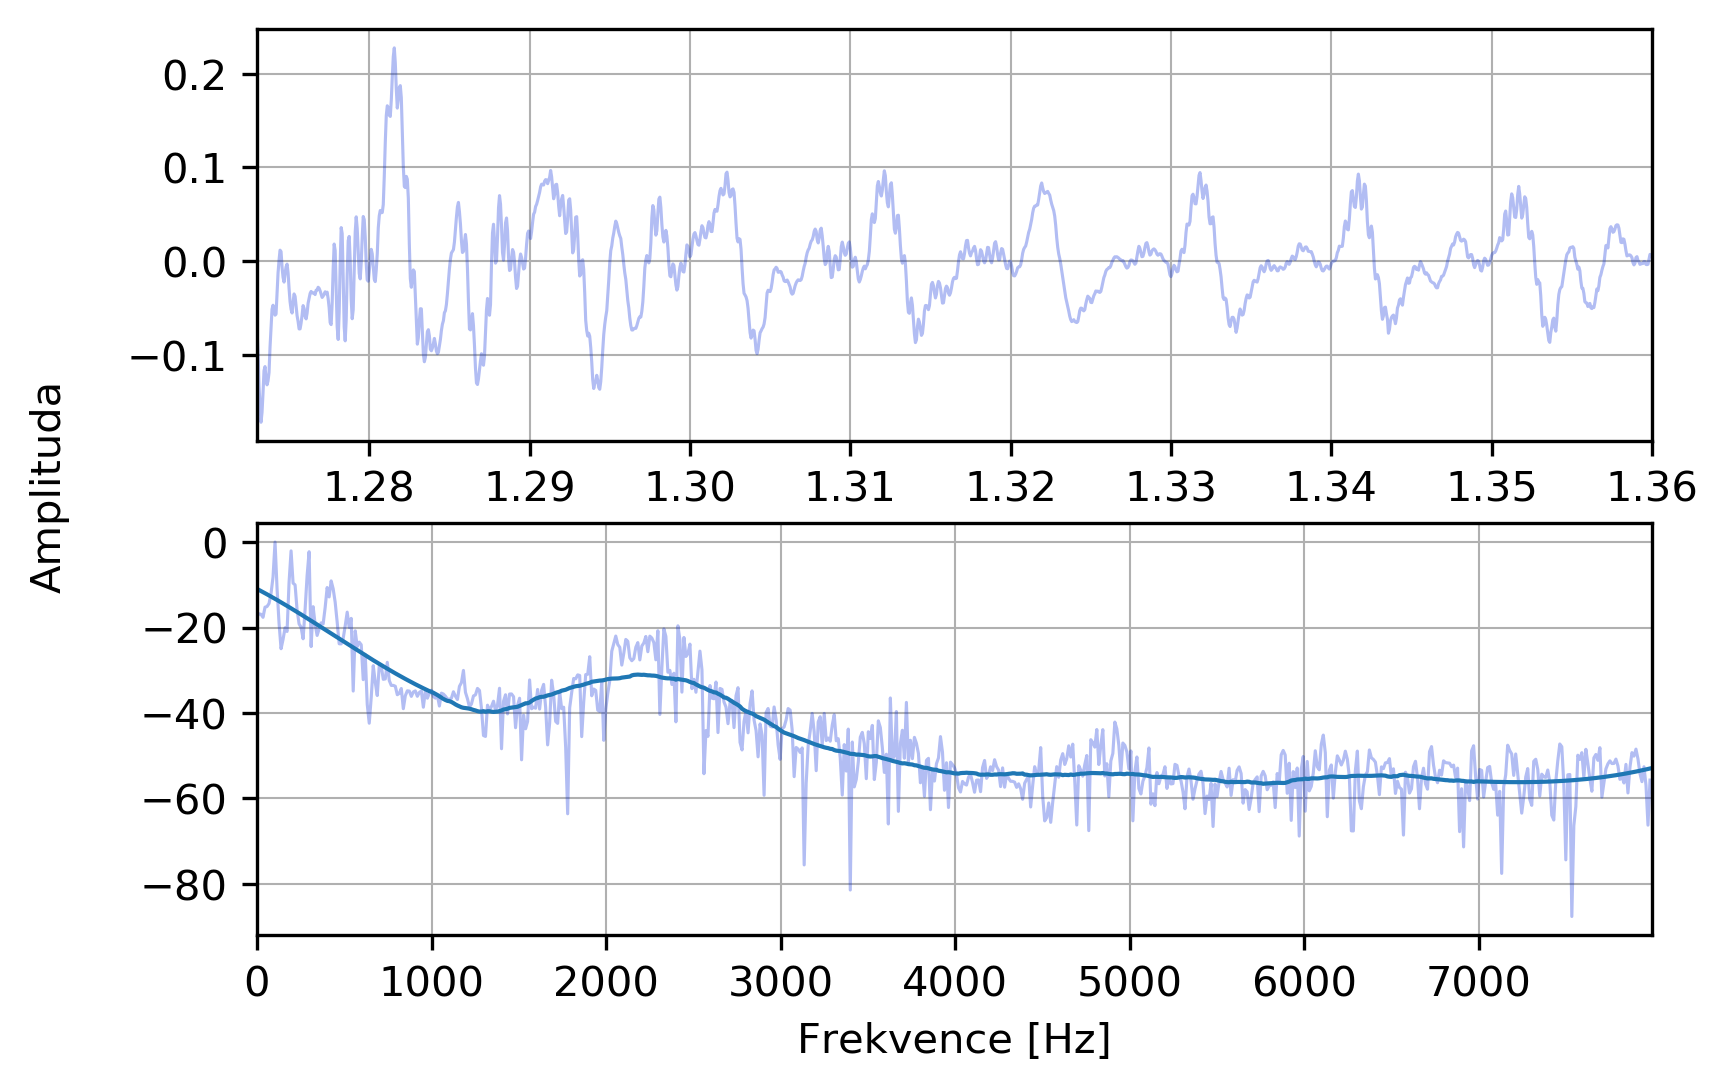
\includegraphics[width=\textwidth]{./ch5-construction/img/signal-normal_g.png}
    \caption{Zdravý řečník}
    \label{fig:construction:phonemes:g:normal}
  \end{subfigure}
  %
  \begin{subfigure}[b]{0.45\textwidth}
    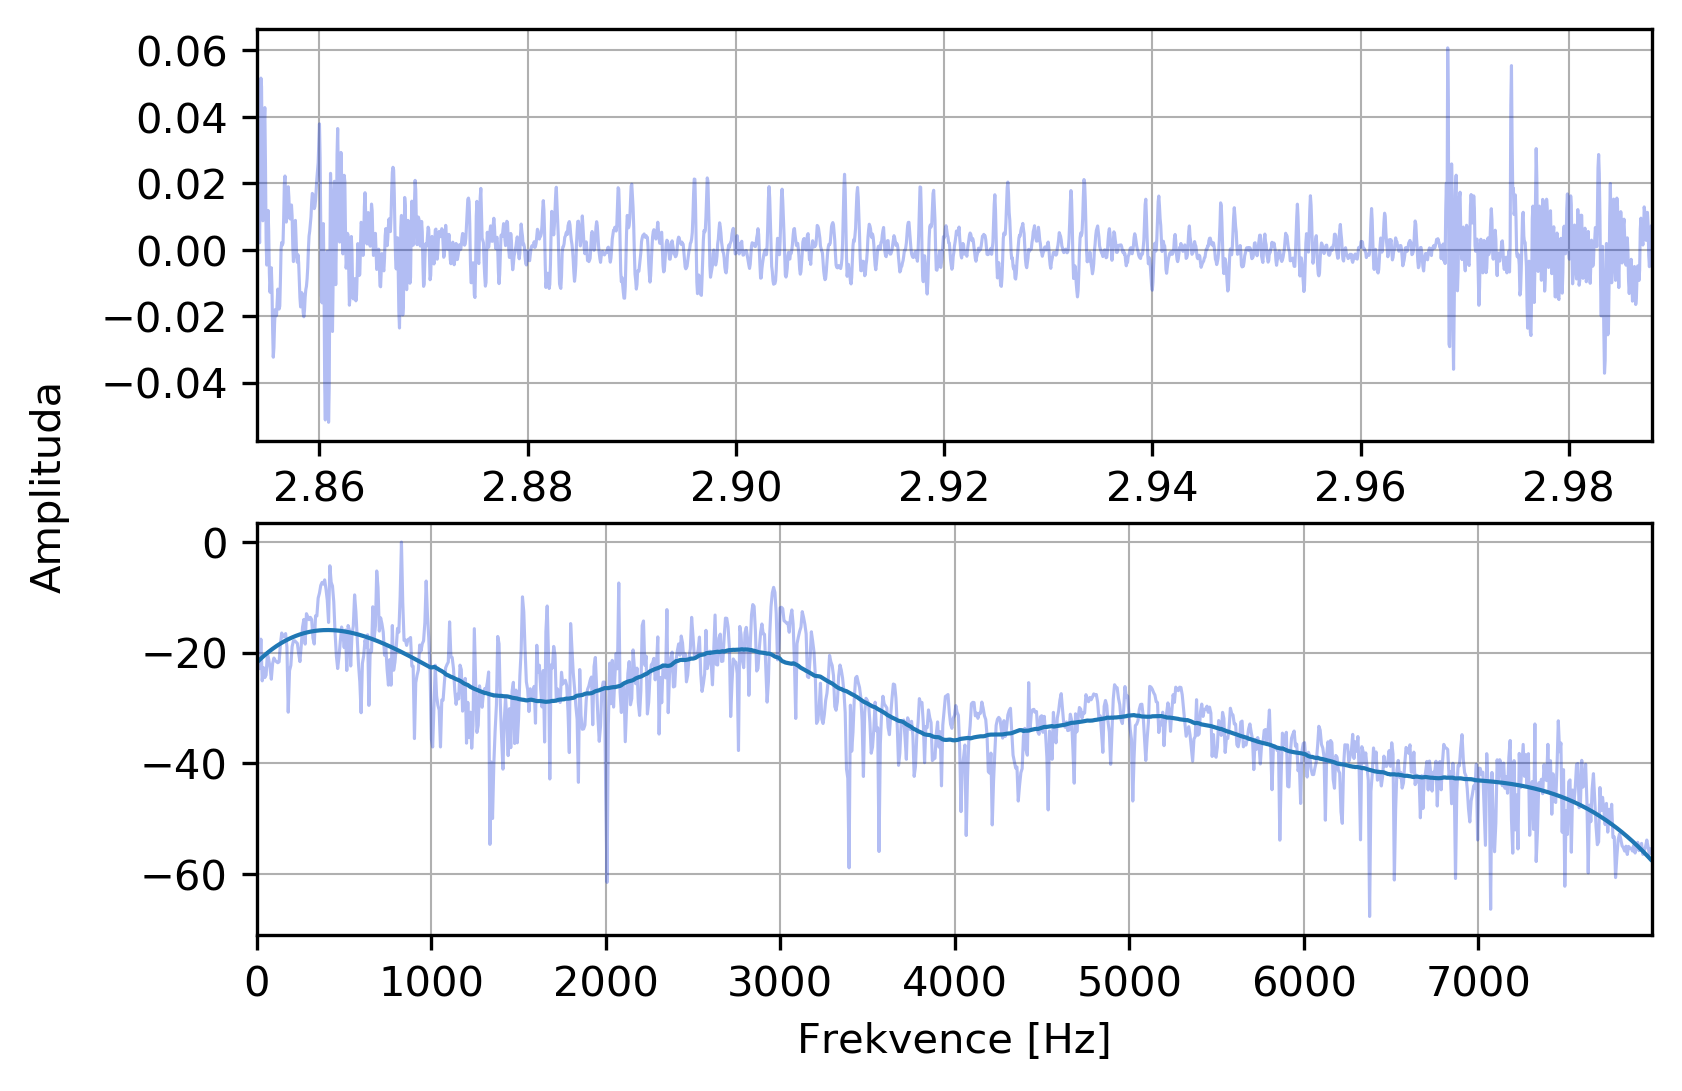
\includegraphics[width=\textwidth]{./ch5-construction/img/signal-el_g.png}
    \caption{EL řečník}
    \label{fig:construction:phonemes:g:el}
  \end{subfigure}
  \caption[Průběh amplitudy fonému $/g/$ zdravého a EL řečníka.]{Průběh amplitudy fonému $/g/$ v~časové a frekvenční oblasti fonému u~zdravého a EL řečníka.}
  \label{fig:construction:phonemes:g}
\end{figure}

Posledním ukázkovým fonémem je již zmiňované $/\check{c}/$.
Jedná se o neznělý foném, který vzniká přiložením jazyku  k~zadní části horního patra.
Tím je zadržen vzduch v~dutině ústní a vzniká krátká pauza.
Uvolněním pak dochází  k~explozi a vytvoření zvuku \cite{Psutka2006}.
Do produkce se nezapojují hlasivky a produkovaný zvuk by měl být dostatečně intenzivní, aby nebyl v~případě EL řečníka tolik neovlivněn případným EL.
Tím pádem by měl být průběh signálu u obou řečníků podobný a to jak v~časové, tak i ve frekvenční oblasti, viz obr. \ref{fig:construction:phonemes:c}.

\begin{figure}[htpb]
  \centering
  \begin{subfigure}[b]{0.45\textwidth}
    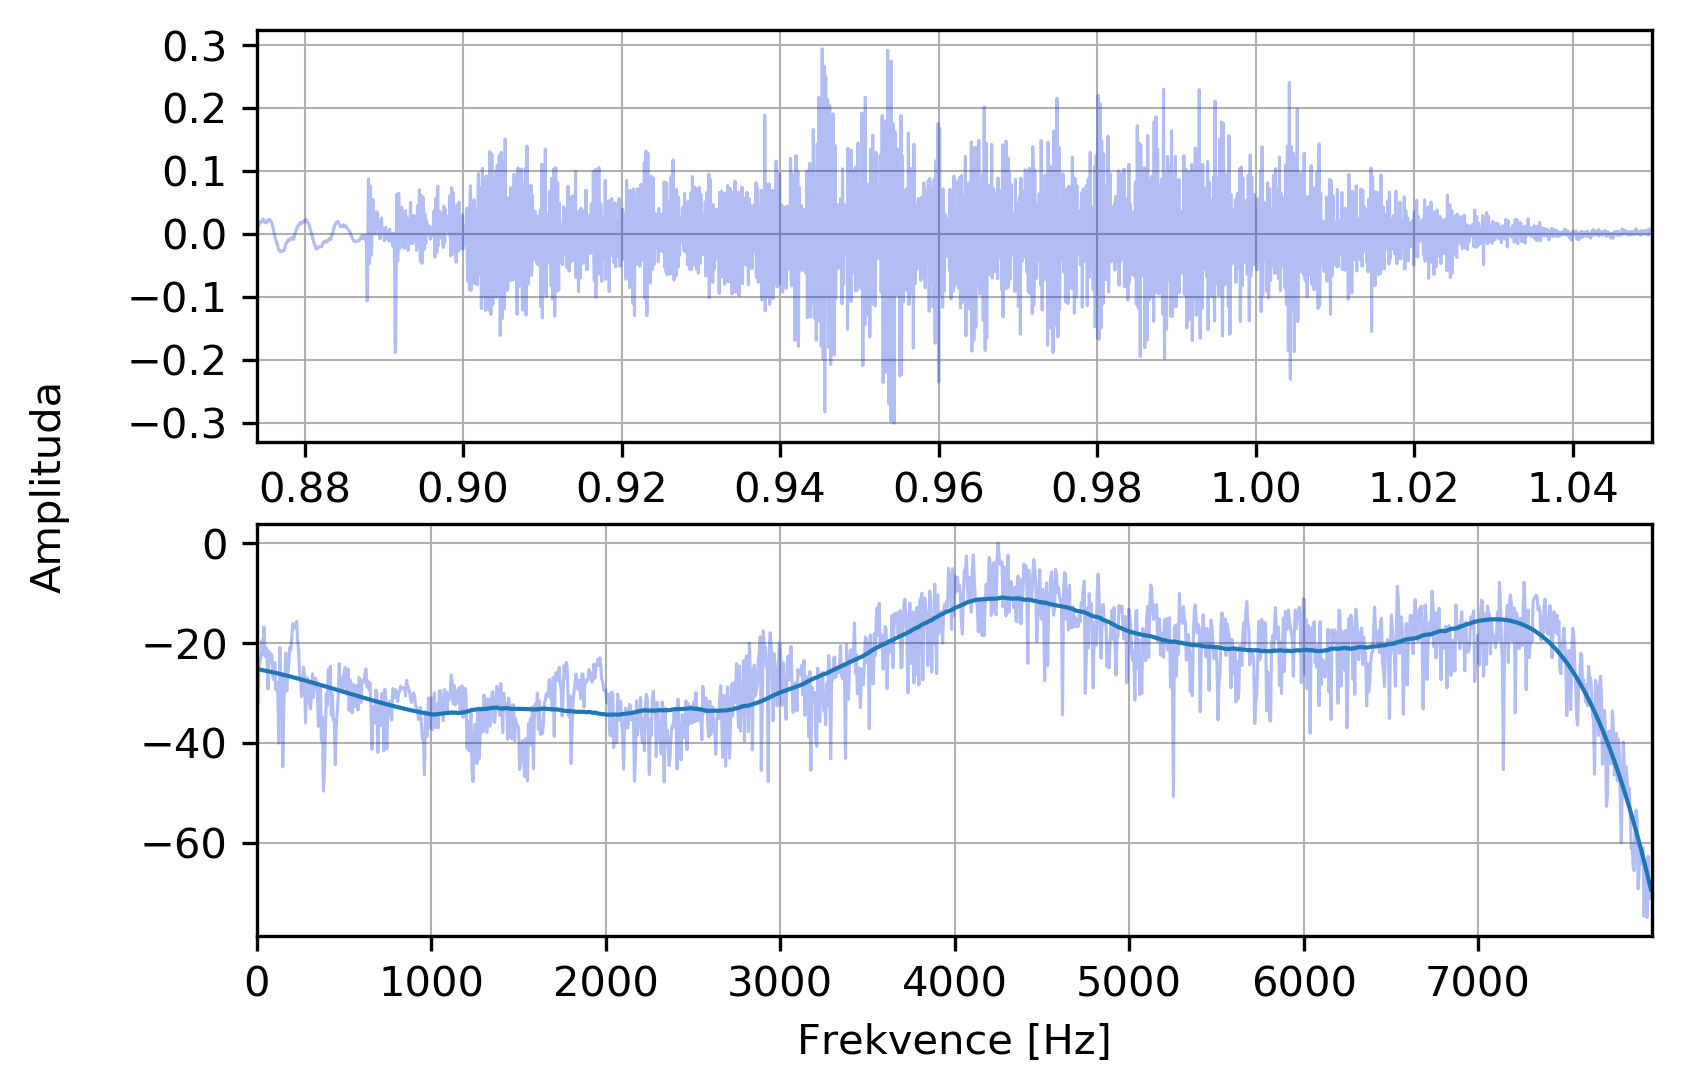
\includegraphics[width=\textwidth]{./ch5-construction/img/signal-normal_c.png}
    \caption{Zdravý řečník}
    \label{fig:construction:phonemes:c:normal}
  \end{subfigure}
  %
  \begin{subfigure}[b]{0.45\textwidth}
    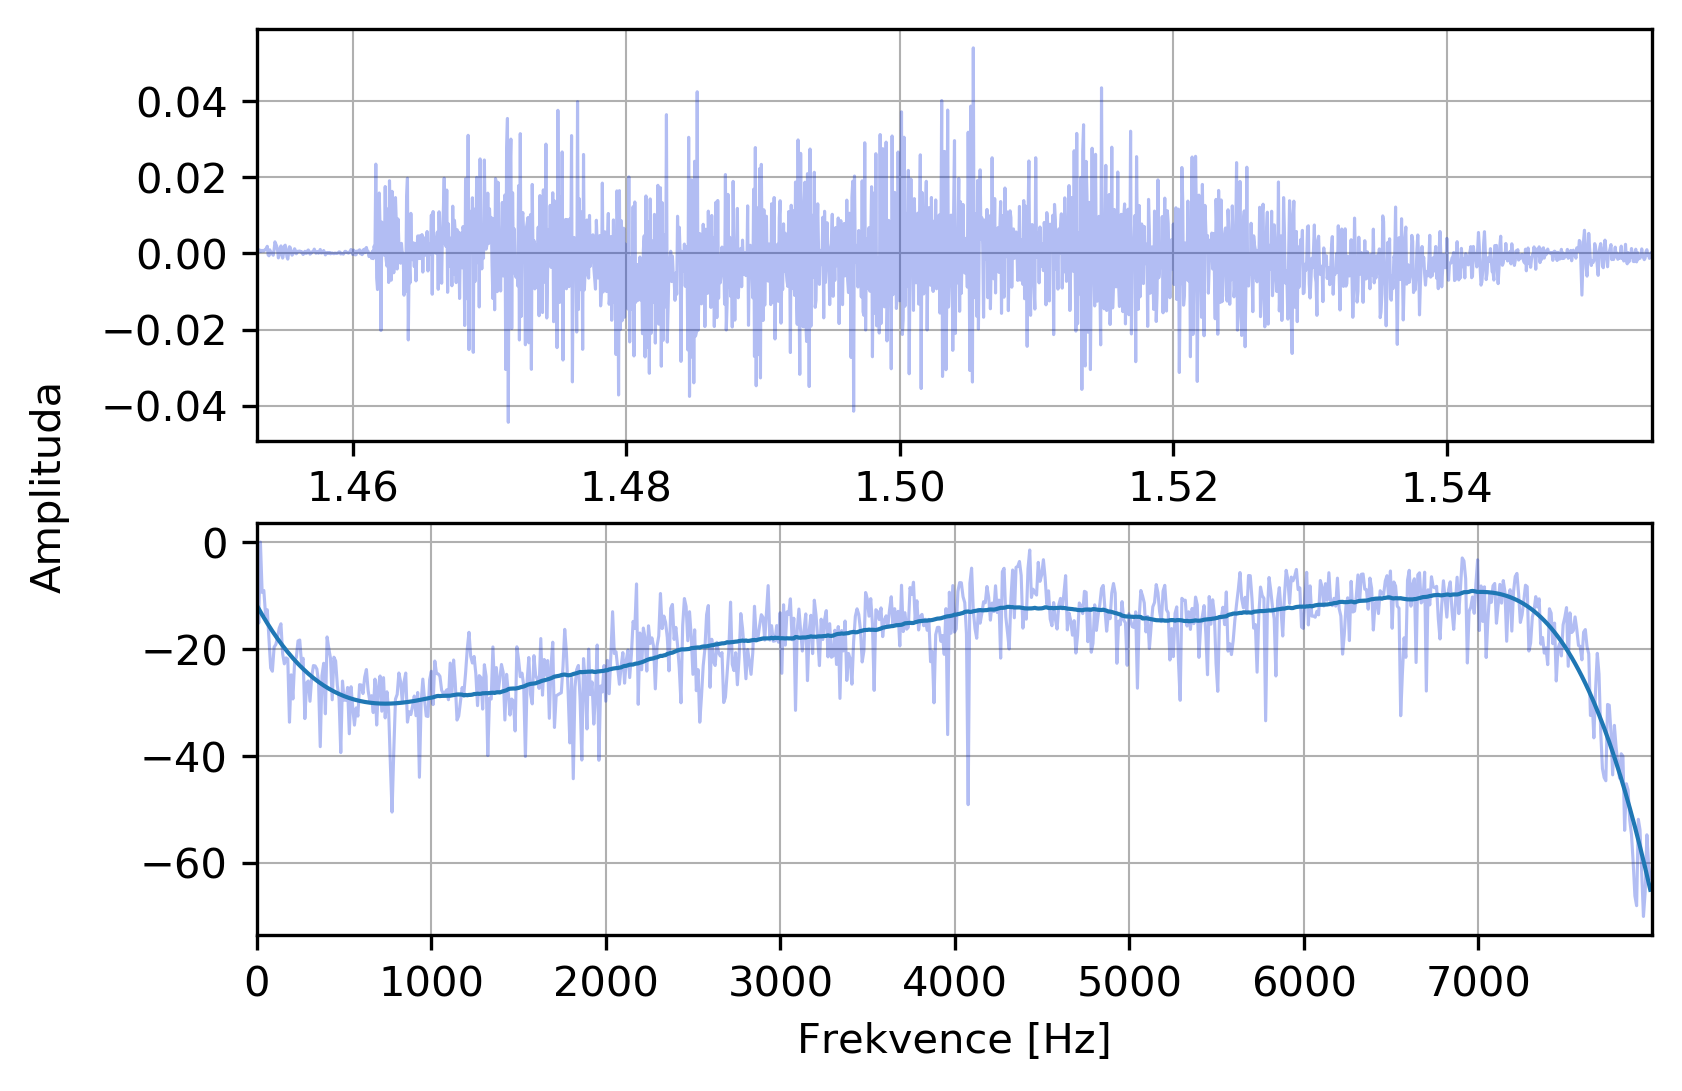
\includegraphics[width=\textwidth]{./ch5-construction/img/signal-el_c.png}
    \caption{EL řečník}
    \label{fig:construction:phonemes:c:el}
  \end{subfigure}
  \caption[Průběh amplitudy fonému $/\check{c}/$ zdravého a EL řečníka.]{Průběh amplitudy fonému $/\check{c}/$ v~časové a frekvenční oblasti fonému u~zdravého a EL řečníka.}
  \label{fig:construction:phonemes:c}
\end{figure}

Z doposud provedené analýzy plyne, že EL řeč je v~mnoha charakteristikách odlišná od té produkované zdravým řečníkem.
Zejména ve frekvenční oblasti (obr. \ref{fig:construction:phonemes:k} a \ref{fig:construction:phonemes:g}) jsou výše uvedené rozdíly patrné.
% Tento fakt nepochybně přispívá  k~tomu, že standardní obecné modely rozpoznávání řeči nedosahují takové přesnosti jako v~případě běžné promluvy, viz dále.

% \csvautotabular{./ch5-construction/test.csv}
